\documentclass[12pt]{article}
\setlength{\oddsidemargin}{0in}
\setlength{\evensidemargin}{0in}
\setlength{\textwidth}{6.5in}
\setlength{\parindent}{0in}
\setlength{\parskip}{\baselineskip}

\usepackage{amsmath,amsfonts,amssymb,bm,graphics,pgfplots,framed,dsfont}
\usepackage[scale=0.75,top=1cm,bottom=3cm]{geometry}

\begin{document}

\textbf{Minh Anh Nguyen }\\
\textbf{Discrete Math\hfill Assignment-7}

\hrulefill

\begin{enumerate}

  \item Refer to Definition 1.10. Show that the divisibility relation | makes the set N of natural numbers a partially ordered set.\\
  \textbf{Reflexivity:}\\
  Because every number $x \in N$ can divides itself. Hence, the divisibility relation is reflexive.\\
  \textbf{Transitivity:}\\
  If $a|b$ and $b|c$ for $a,b,c \in N$. Then $b = a.k$ and $c = b.m$ and $c = a.k.m$. Therefore, c can divides a. Hence, the relation $|$ is transitivity.\\
  \textbf{Antisymmetry:}\\
  If $a|b$ with $a,b \in N$, $a < b$. Hence, a cannot divide a. Therefore, the relation $|$ is antisymmetric.\\
  Hence, the relation $|$ is a partially order set.
  \item Explain why the divisibility relation $|$ does not define a partially ordering on the set Z of integers.\\
  For $x = -1$ and $y = 1$. $x|y$ and also $y|x$. Hence, the relation is not antisymmetric. Therefore, the relation is not a partially ordering set.
  \item Consider the poset $(N,|)$. Are there any minimal elements? Are there any maximal elements? Explain.\\
  Because N = \{1,2,3,4,...$\infty$\}. The minimal element is 1 and there is no maximal elements.
  \item Let A = \{a,b,c,...z\}. In the poset(P(A), $\subset$), find a pair of incomparable elements.\\
  A pair of incomparable elements is (\{a,b,c\},\{d,e,f\}).
  \item Let $W$ be the set of all web pages. For $x, y \in W$, let $x R y$ if you can navigate from $x$ to $y$ by following links (Let's say it always possible to "navigate" from a page to itself; just do nothing.) Explain why R is not a partial ordering.\\
  Let $x,y \in W$, it is possible to navigate from x to y and from y to x. Hence, xRy and yRx. Therefore, R is not antisymmetric and not a partially ordering set.
  \item Let a relation R be defined on the set of real numbers as follows:
  \[xRy \Leftrightarrow 2x + y = 3\]
  Prove that this relation is antisymmetric.\\
  Let: $y = 3 - 2x$\\
  For $yRx$:
  \[yRx \Leftrightarrow 2y + x = 3\]
  \[2(3-2x) + x = 3\]
  \[6-4x + x = 3\]
  \[-3x = -3\]
  \[x = 1\]
  \[y = 3 - 2(1) = 1\]
  Hence, x = y. \\
  Therefore, the relation is antisymmetric.
  \item Explain why the relation R on \{0, 1, 2, 3\} given by
  \[R = \{(0,0),(1,1),(2,2),(3,3),(0,1),(1,2),(2,3),(0,2)\}\]
  is not a partial ordering on \{0, 1, 2, 3\}. Be specific.\\
  Because 1R2 and 2R3 but there is no relation between 1 and 3. Hence, the relation R is not transitive. Therefore, the relation is not a partially ordering set.
  \item Explain why the relation R on \{0, 1, 2, 3\} given by
  \[R = \{(0,0),(1,1),(2,2),(3,3),(0,1),(1,2),(0,2),(2,1)\}\]
  is not a partial ordering on \{0, 1, 2, 3\}. Be specific.\\
  Because 1R2 and 2R1, the relation is not fully antisymmetric. Hence, the relation is not partial ordering.
  \item The Hasse diagram below defines a partial ordering on the set \{0, 1, 2, 3\}. Give the set of ordered pairs corresponding to this relation.
  \begin{center}
    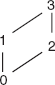
\includegraphics[scale=0.8]{img/img-0.png}
  \end{center}
  \[R = \{(0,1),(1,3),(0,2),(2,3),(0,3),(0,0),(1,1),(2,2),(3,3)\}\]
  \item The Hasse diagram below defines a partial ordering on the set \{0, 1, 2, 3\}. Give the set of ordered pairs corresponding to this relation.
  \begin{center}
    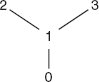
\includegraphics[scale=0.8]{img/img-1.png}
  \end{center}
  \[R = \{(0,1),(0,2),(0,3),(1,2),(1,3),(0,0),(1,1),(2,2),(3,3)\}\]
  \newpage
  \item The divides relation “$|$” defines a partial ordering on the set \{1, 2, 3, 6, 8, 10\}. Draw the Hasse diagram for this poset. What are the maximal elements?
  \begin{center}
    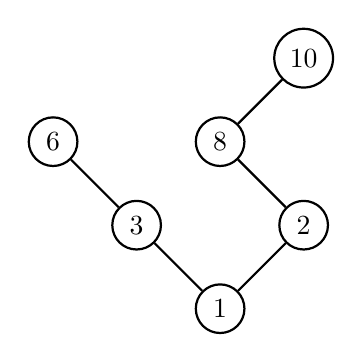
\begin{tikzpicture}[node distance={15mm}, thick, main/.style = {draw, circle}] 
        \node[main] (1) {$1$}; 
        \node[main] (2) [above right of=1] {$2$}; 
        \node[main] (3) [above left of=1] {$3$}; 
        \node[main] (4) [above left of=3] {$6$}; 
        \node[main] (5) [above right of=3] {$8$};
        \node[main] (6) [above right of=5] {$10$}; 
        \draw(1) -- (3);
        \draw(1) -- (2);
        \draw(3) -- (4);
        \draw(2) -- (5);
        \draw(5) -- (6);
        \end{tikzpicture} 
  \end{center}
  The maximal elements are 6 and 10.
  \item Let S = \{1, 2, 3, 5, 10, 15, 20\}. It is a fact that (S, $|$) is a poset. Draw its Hasse diagram.
  \begin{center}
    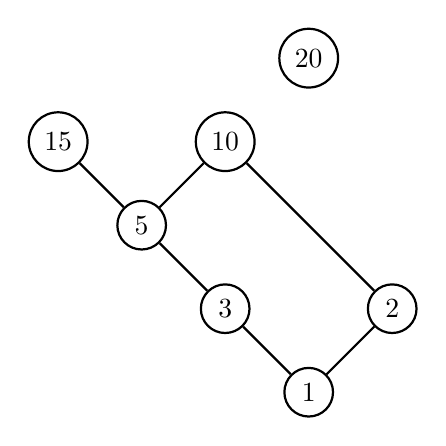
\begin{tikzpicture}[node distance={15mm}, thick, main/.style = {draw, circle}] 
        \node[main] (1) {$1$}; 
        \node[main] (2) [above right of=1] {$2$}; 
        \node[main] (3) [above left of=1] {$3$}; 
        \node[main] (4) [above left of=3] {$5$}; 
        \node[main] (5) [above right of=4] {$10$};
        \node[main] (6) [above left of=4] {$15$};
        \node[main] (7) [above right of=5] {$20$}; 
        \draw(1) -- (3);
        \draw(1) -- (2);
        \draw(3) -- (4);
        \draw(2) -- (5);
        \draw(4) -- (5);
        \draw(4) -- (6);
        \end{tikzpicture} 
  \end{center}



       
\end{enumerate}
\end{document}